%%%%%%%%%%%%%%%%%%%%%%%%%%%%%%%%%%%%%%%%%%%%%%%%%%%%%%%%%%%%%%%%%%%%%%%%%%%%%%%%

\documentclass[letterpaper, 11 pt, onecolumn]{article}

\linespread{1.0}
\usepackage{tgpagella}
\usepackage{url}
\usepackage{hyperref}

\usepackage[dvips]{color}

\usepackage{pslatex}
% \usepackage{nopageno}
\usepackage{enumitem}
\setlist{itemsep=0em, topsep=0em}
\usepackage[left=1in,right=1in,top=1in,bottom=1in]{geometry}

\usepackage{tabularx}
%\usepackage{hangcaption}
\usepackage[font=footnotesize]{caption}
\usepackage[final]{graphicx}
%\DeclareGraphicsExtensions{.eps,.ps,.PS,.EPS}
\usepackage{epsfig}
%\usepackage{subfig}
\usepackage{tikz}

\usepackage{amsmath}
\usepackage{amssymb}
\usepackage{fancyhdr}
\usepackage{tikz}
\usetikzlibrary{automata,positioning}

%\usepackage{xspace}
\usepackage{cite}
\usepackage{url}
\usepackage[letterpaper]{}
\usepackage{epstopdf}
\usepackage{authblk}
\usepackage{lineno}
\usepackage{todonotes}
\usepackage{soul}
\usepackage[utf8]{inputenc}
\usepackage[english]{babel}
%\usepackage[font=footnotesize,labelfont=bf]{caption}
\usepackage[font=small,labelfont=bf]{caption}
\usepackage{pgfgantt}
\usepackage[numbers,sort&compress]{natbib}

\usepackage[compact]{titlesec}
\usepackage{subcaption}

\usepackage{titling}
\setlength{\droptitle}{-5em}   % This is your set screw
\setlength{\belowcaptionskip}{-10pt}
\usepackage{titlesec}
\titlespacing*{\section}{0pt}{0.4\baselineskip}{0.4\baselineskip}
\titlespacing*{\subsection}{0pt}{0.4\baselineskip}{0.4\baselineskip}
\titlespacing*{\subsubsection}{0pt}{0.4\baselineskip}{0.4\baselineskip}
\setlist[itemize]{leftmargin=*}

\setcounter{topnumber}{2}
\setcounter{bottomnumber}{2}
\setcounter{totalnumber}{4}
\renewcommand{\topfraction}{0.85}
\renewcommand{\bottomfraction}{0.85}
\renewcommand{\textfraction}{0.15}
\renewcommand{\floatpagefraction}{0.8}
\renewcommand{\textfraction}{0.1}
\setlength{\floatsep}{5pt plus 2pt minus 2pt}
\setlength{\textfloatsep}{5pt plus 2pt minus 2pt}
\setlength{\intextsep}{5pt plus 2pt minus 2pt}

% for comments
\newcommand{\zhi}[1]{\textcolor{blue}{ZL: #1}}
\newcommand{\jie}[1]{\textcolor{green}{JF: #1}}
\newcommand{\brian}[1]{\textcolor{magenta}{BZ: #1}}



% \setlist[enumerate]{leftmargin=*}

\titlespacing{\paragraph}{%
  0pt}{%              left margin
  0\baselineskip}{% space before (vertical)
  0.3em}%               space after (horizontal)

\titlespacing{\subsection}{%
  0em}{%              left margin
  0.15\baselineskip}{% space before (vertical)
  0.15\baselineskip}%               space after (horizontal)

% figures with text wrapped around
\usepackage{wrapfig}
\usepackage{titling}
\setlength{\droptitle}{-5em}   % This is your set screw
\setlength{\textfloatsep}{0.8\baselineskip plus 0.2\baselineskip minus 0.5\baselineskip}

\newcommand{\fig}[1]{Fig.~\ref{#1}}
\newcommand{\figs}[2]{Fig.~\ref{#1} to~\ref{#2}\xspace}
\newcommand{\figa}[2]{Fig.~\ref{#1} and~\ref{#2}\xspace}
\newcommand{\eq}[1]{Eq.~(\ref{#1})}
\newcommand{\eqs}[2]{Equations~(\ref{#1}) to~(\ref{#2})}
\newcommand{\eqa}[2]{Equations~(\ref{#1}) and~(\ref{#2})}
% The following packages can be found on http:\\www.ctan.org
%\usepackage{graphics} % for pdf, bitmapped graphics files
%\usepackage{epsfig} % for postscript graphics files
%\usepackage{mathptmx} % assumes new font selection scheme installed
%\usepackage{times} % assumes new font selection scheme installed
%\usepackage{amsmath} % assumes amsmath package installed
%\usepackage{amssymb} % assumes amsmath package installed

\pagestyle{plain}                                                      %%
%%%%%%%%%% EXACT 1in MARGINS %%%%%%%                                   %%
\setlength{\textwidth}{6.5in}     %%                                   %%
\setlength{\oddsidemargin}{0in}   %% (It is recommended that you       %%
\setlength{\evensidemargin}{0in}  %%  not change these parameters,     %%
\setlength{\textheight}{8.5in}    %%  at the risk of having your       %%
\setlength{\topmargin}{0in}       %%  proposal dismissed on the basis  %%
\setlength{\headheight}{0in}      %%  of incorrect formatting!!!)      %%
\setlength{\headsep}{0in}         %%                                   %%
\setlength{\footskip}{.5in}       %%                                   %%
%%%%%%%%%%%%%%%%%%%%%%%%%%%%%%%%%%%%                                   %%
\renewcommand{\refname}{References Cited}                              %%
\bibliographystyle{plain}



\begin{document}


\setcounter{page}{1}

\pagebreak

\begin{center}
	{\Large \bf Measure Human Adaption Level to Robot Teleoperation Interface}\\
    \vspace{4pt}
% 	\renewcommand{\baselinestretch}{1}
   	{\large PI: Zhi Li (Worcester Polytechnic Institute)}
   	% \vspace{4pt}
    % {\large Worcester Polytechnic Institute}
\end{center}

\vspace{1 em}

\paragraph*{\Large Project Summary} 
This project aims to develop novel metrics to measure the level of adaption of human teleoperator to robot teleoperation interface, and to quantitatively compare the usability of various human-robot control interfaces for manufacturing tasks that involve complex motion coordination. In this research, we will setup various teleoperation interfaces to control the hand-arm coordination, bimanual coordination and loco-manipulation of a mobile humanoid robot, and (2) the coordination of multi-arm and macro-micro structure of precise manipulator robotic system. 
In addition to the available human, robot and task performance metrics, we propose novel metrics, including the \textit{complexity}, \textit{predictability}, \textit{intuitivity} and \textit{robust to uncertainty}, to measure the low-level motor skills of a teleoperator exhibited through the teleoperation interface. We further compose abstract representation of the motion coordination plan, and infer the \textit{reward function} of the teleoperator in decision-making. Our proposed method will be used to evaluate the skill progression from novice to expert, and to identify the milestones and thresholds in robot teleoperation skill development. The proposed project will inform the development of transparent interface for controlling complex robotic system, and will provide guideline to the development of intelligence robot assistance to reduce the control and learning efforts of manfacturing workers.  


% the teleoperated motion coordination. 


% measure the human-robot collaboration performance in teleoperation by

% of low-level motion primitives and high-level task plan in the




% % Specifically, we decompose the decompose the teleoperated robot motion coordination to identify the set the low-level motion primitives for each robot component and their frequent combination. We further construct the high-level representation of the teleoperated robot motion coordination using robot option symbols (the abstraction of the motion primitives). 

% % and their ( abstract robot-task states   

% evaluate the level of decompose the motion coordination  
% Planning and control of motion coordination of a complex robotic system in cluttered human environment requires human-level manipulation dexterity and decision-making intelligence and thus far can only be reliably achieved under direct teleoperation. The performance of human-robot teleoperation system depends primarily on the teleoperator's expertise, which reflects how well the teleoperators can utilize the motion and perception capabilities of their remote robot surrogate given the motion/perception mapping defined by the teleoperation interface. Studies on teleoperation interface design have proposed methods that facilitate intuitive motion mapping, and reduce perception/control workload and discomfort. However, little research has been conducted to measure and compare the coordinated motions teleoperated through various interface by the quality of low-level motor skills and high-level decision-making. Performance metrics haven been developed for human and robot independently without considering their task-dependent and time-varying synergy. Thus, through this project we aim to develop and validate metrics for measuring the adaption level of human motor control and decision-making strategy to a teleoperated robotic system in complex motion coordination.  

% % adapt human motion coordination strategies to their remote robot surrogates.

% To meet this need, we propose to learn from novice- and expert-demonstration of the motion coordination, compare the demonstrations by their low-level motion primitive models and high-level motion plan model, to learn the features for measure the performance of human-robot teleoperation system. The demonstrations are collected from a mobile humanoid robot controlled through various teleoperation interfaces. Standard human and robot performance metrics are used to evaluate meta performance of human-robot teleoperation system, and quantify the skill levels of novices and experts. Dynamic movement primitives (DMP) and Gaussian Mixture Model/Gaussian Mixture Regression (GMM/GMR) are used to model the motion coordination within robotic system, while Probabilistic Movement Primitives (Pro-MP) is used to model the motion coordination between robotic system and environment. Novel metrics for the regularity, variability, complexity of the motion primitives are proposed as the features to characterize the low-level motor skills. Machine learning methods are used to identify the principle components and characteristic synergy in the motion primitive feature space, to compare low-level motor skills across tasks, teleoperation interfaces, and users. To model the high-level task plan, we abstract the critical robot states in motion coordination  and motion primitives for state transition to symbols, and use these symbols to construct an abstract task space graph. The costs of graph nodes and edges, which denote the abstract states and state-transition motion primitives, are assigned by weighting the teleoperator's operation efforts, efficiency, frequency and success ratio. Given the abstract motion coordination representation, we propose several optimization criteria, derived from several hypotheses of the human motion coordination strategies, and compose a reward function with unknown weighting coefficients. The weighting assignment learned from demonstrated high-level task plan can be used for evaluate and compare a teleoperator's motion coordination control strategies. 

% Our proposed methods can be generalized to evaluate the teleoperated motion coordination for various complex robotic systems. Previous research at WPI human-inspired robotics lab has integrated a mobile humanoid robots which supports teleoperation from multi-modal interfaces. The proposed model user study, model development and data analysis can be accomplished in one year. Future work may include (1) extending the proposed project to evaluate the motion coordination of the multi-arm surgical robot (platform available at WPI AIM lab) and swarm robot system (available at WPI NEST lab), as well as available industrial robot platform at research lab at NIST; and (2) using the developed evaluation metrics to study the motor skill progression from novice to expert; and (3) shift the control between human teleoperator and intelligent tele-operated robot based on learning of high-level motion coordination strategies and low-level coordinated motion primitives from human teleoperators. 





% Take the teleoperation of mobile humanoid nursing robot for instance: the motion coordination involved in patient-caring tasks includes , and may extend to the coordination of end-effectors for sensing and action. 

% skill acquisition efforts of novice worker to  

% Tele-operated robotic systems extend the physical capabilities of medical and industrial workers to perform  tasks in remote, inaccessible, and/or hazardous environments. 

% tasks that require human-level manipulation dexterity and decision-making intelligence are infeasible through autonomous control, yet can be accomplished under direct (tele)operation. To freely and efficiently control their remote surrogates, human workers need to devote significant efforts to learn the motion and perception mapping defined by the (tele)operation interface. To address this needs, we propose to investigate the physical and cognitive interactions between human workers and (tele)operation interfaces, and develop a user interface to support intuitive robot control and multi-modality cognitive augmentation. Our proposed project aims to (a) reduce the teleoperation control effort in dexterous and coordinated manipulation tasks, and to (b) facilitate novice workers to acquire the fine motor skills for operating complicate robotic systems to work on various manufacturing tasks. To this end, we propose to investigate theories and technologies that (1) Shift the boundary between direct teleoperation and autonomous control based on the physical and mental status of the operator, (2) Infer human teleoperator's contextual intent based on the knowledge of manipulation tasks and human motions, in order to automate low-level robot actions. 

% \vspace{0.5 em}

% \paragraph*{\Large Intellectual Merit}
% This project addresses how multi-modality cognitive feedback affects human motor behavior and motor learning process. Specifically, we will experimentally study in teleoperated manipulation tasks that requires simultaneous control of multiple robot components, such as loco-manipulation, bimanual coordination, arm-hand-finger coordination. For \textbf{expert workers}, we focuses on \textit{how human decision-making and task operation can be affected by single- and multi-modality cognitive feedback, and investigate methods for intuitive and integrated representation of task information and cognitive feedback}. For \textbf{novice workers}, we will focus on \textit{how multi-modality cognitive feedback affects the explicit and implicit learning of dexterous and coordinated manipulation motor skills}, as well as \textit{when and how to provide high-level/abstract cognitive feedback (e.g., verbal/text instructions, numbers, etc.) and low-level intuitive cognitive feedback (e.g., colors, shapes, sounds, tactile and forces, etc.) to facilitate the interactive and associated explicit and implicit motor learning}. Our proposed research is unique for it will develop a unified framework that integrate the model-based and model-less robot learning methodologies to reveal the underlying principles of the associated implicit and explicit human motor learning processes. The enhanced understanding of the cognitive and physical interactions between human worker and teleoperation interfaces further leads to novel techniques for user-adaptive cognitive augmentation and decision-making assistance, which leverages ``cloud wisdom'' and adjust the human-robot control efforts based on a human worker's intents, physical/mental states, and skill level. 

% % to robot learning that acquire motion and task knowledge through  (e.g., reinforcement learning with explicit reward function v.s. learning through convolutional neural network). Inspired by how human can develop situational awareness and motor skills through intuitive and abstract cognitive feedback and augmentation, we will further develop novel robot teaching methodologies for that leverage human-guided robot interactions with environments and demonstrations/critiques from human teachers. 


% % By investigating the underlying principles of the cognitive and physical interaction between the human worker and teleoperation interfaces, we will advance the technologies for user-adaptive cognitive augmentation to facilitate novice workers to build their situational awareness and master the motion mapping between the input interfaces and their physical embodiments in the tasks. Towards the seamless integration of human and (tele-)operated robotic systems, our research will further investigate shared-autonomous control methods for adjusting the human-robot control efforts based on human worker's skill level and physical/mental states. 

% % We will also investigate how to utilize the teleoperation interface as an efficient robot teaching interface, to relieve workers from repetitive low-level teleoperation. 


% % Towards the seamless integration of human and (tele-)operated robotic systems, we will further investigate shared-autonomous control methods for adjusting the human-robot control efforts based on human worker's skill level and physical/mental states. We will also investigate how to utilize the teleoperation interface as an efficient robot teaching interface, to relieve workers from repetitive low-level teleoperation. 

% % This project aims to discover the new knowledge of how multi-modality cognitive feedback affects explicit and implicit learning processes of coordinated manipulation motor skills, and develop novel methodologies for 

% % how this knowledge can be used to (1) 

% % develop robot control interface that integrates intuitive and abstract multi-modality  to provide user-adaptive   

% % Specifically, we will experimentally study in teleoperated manipulation tasks, how human decision-making and task operation can be affected by single- and multi-modality cognitive feedback, and investigate methods for intuitive and integrated representation of task information and cognitive feedback, to reduce an expert worker's the physical and mental efforts. For novice workers, we will focus on how multi-modality cognitive feedback affects the explicit and implicit learning of dexterous and coordinated manipulation motor skills, as well as when and how to provide high-level/abstract cognitive feedback (e.g., verbal/text instructions, numbers, etc.) and low-level intuitive cognitive feedback (e.g., colors, shapes, sounds, tactile and forces, etc.) to facilitate the interactive and associated explicit and implicit motro learning. By investigating the underlying principles of the interaction between the human worker and teleoperation interfaces, we will develop user-adaptive cognitive augmentation to facilitate novice workers to build their situational awareness and master the motion mapping between the input interfaces and their physical embodiments in the tasks. Towards the seamless integration of human and (tele-)operated robotic systems, we will further investigate shared-autonomous control methods for adjusting the human-robot control efforts based on human worker's skill level and physical/mental states. We will also investigate how to utilize the teleoperation interface as an efficient robot teaching interface, to relieve workers from repetitive low-level teleoperation. 



% \vspace{0.5 em}

% \paragraph*{\Large Broader Impacts}
% Our research will directly and primarily benefit industrial workers that operate tele-manufacturing robotic system, and will have boarder impacts on a wide range of workers that need to master the skill of operating complex human-machine interfaces for direct control and robot teaching, such as tele-surgery, tele-nursing, and shared-autonomous driving. By improving the usability of teleoperation interface, we aim to improve the availability of healthcare, industrial, and social service labor, and provide capable surrogates for military and medical personnels in tedious, repetitive, and dangerous tasks. It will also lead towards affordable robotic solutions can provide assistance and job opportunities to wider populations. Our research will also synergize with graduate and undergraduate education for students from engineering, medical, and nursing schools. It will also actively engage K-12 students, REU students in summer research and the general public in open lab activities. 

% Through robot-mediated interactions, develops robot motion intelligence in a multi-agent, highly-interactive context. 



% to navigate in cluttered human environments and perform a wide variety of dexterous manipulation tasks with minimal human control. Our key idea is to develop a unified framework for lifelong learning and fast, context-based intent and in simultaneous multi-lateral physical human-robot interactions. In such scenarios, the nursing robot participates in a patient-caring task, while learning when and how to intervene in the robot-mediated collaboration between its remote teleoperator and on-site human partners. By observing human experts, the nursing robot will also establish hierarchical knowledge of natural coordinated human motions and human-human interactions, and metrics for evaluating task performance and motion capabilities. Such motion knowledge and metrics will be used to evaluate the level of skills of novice teleoperators, patients and partner nurses, and adjust the level of assistance provided to maintain nursing task performance and fluency of human-robot collaboration. 

  
% \vspace{0.5 em}

% \paragraph*{\Large Intellectual Merit}
% Our proposal aims to address the need for \textit{\textbf{customizable robot motion intelligence}}, and to \textit{\textbf{lower the barriers}} for medical personnel to synergize with tele-robotic technologies. Our proposed framework enables a tele-robotic system to develop and evolve its contextual motion intelligence through lifelong interactions with human experts, and apply its motion intelligence to provide user-adaptive assistance to reduce learning and operation effort for novice teleoperators.   



% \vspace{0.5 em}

% \paragraph*{\Large Broader Impacts}
% This project envisions broader impacts on a wide range of mobile humanoid robots for medical, industrial, and social service tasks. Our research efforts will enable these robots to interact simultaneously and physically with both the teleoperator and end users, and reconcile their intents to achieve natural, fluent, and intimate collaboration.
% % PM: I changed this to singular "barrier" to make the claim a bit less grand? Feel free to change back if desired.
% We aim to remove a major barrier that prevents robots from integrating into human society as capable and socially acceptable peers. By improving the usability of dexterous robotic manipulators under direct teleoperation and shared-autonomous control, this project may also lead to improved availability of healthcare, industrial, and social service labor, and provide surrogates for military and medical personnel for tedious, repetitive, and dangerous tasks. It will lead towards affordable robotic solutions for hospital and home care that can provide long-term assistance to aging and disabled populations. Our research will also synergize with graduate and undergraduate education for students from engineering, medical, and nursing schools, and will actively engage K-12 students and the general public. 

% \vspace{2 em}
% \noindent
% \textbf{Keywords} --- Customizability, Lowering Barriers, Learning, Human-Robot Interaction, Medical

\pagebreak
\setcounter{page}{1}
%-------------------------------------------------------------------------
\section{Research Overview, Motivations and Objectives}\label{sec:intro}
%-------------------------------------------------------------------------

Tele-operated robotic systems enable workers to perform manufacturing and maintenance tasks in remote, inaccessible, and/or hazardous environments. Complex and risk-sensitive tasks that require dexterous motion coordination skills and decision-making intelligence cannot be fully automated, yet can be reliably accomplished under human control. Given a specific task and robotic system, the performance of human-robot teleoperation depends on the usability of the teleoperation interface and the teleoperator'expertise. The state-of-the-art robotic systems, including humanoid and multi-robot systems, have been endowed with the motion capabilities that conventional teleoperation interfaces cannot fully utilize. Teleoeprating such robotic systems are particularly difficult when the tasks involve mutli-component, multi-arm and multi-robot coordination. Given the complexity of robotic systems and tasks, novel measurement metrics for interface usability and human performance need to be developed to inform the teleoperation interface design and teleoperation skill development for complex robot motion coordination. 

% Metrics for human performance in simple tasks are not sufficient to evaluate the teleoperation skill of  

% Previous research have proposed novel teleoperation interface design that facilitate intuitive motion/perception mapping, and reduce physical and cognitive workload and discomfort.

To meet this need, we propose a novel perspective to understand the performance of human-robot teleoperation. We propose a hierarchical framework to \underline{model the structure of teleoperated robot motion}, such that the evaluation of low-level motor skill can be separated from that of high-level task planning. Based on this framework, we propose novel metrics, including \textit{Outcome Predictability}, \textit{Mapping Sensitivity}, \textit{Operation complexity}, to \underline{measure the usability of teleoperation interfaces}. These metrics evaluates the robot control interface's capabilities of mapping the low-level motor skill and high-level task plan from human to the controlled robotic systems. We use these metrics to compare several conventional and novel control interfaces for a mobile humanoid robot (see \fig{NursingTask}), in general-purpose tasks that involve arm-hand coordination, bimanual coodination, loco-manipulation, and human-robot collaboration. 

% \begin{wrapfigure}{r}{0.75\linewidth}
\begin{figure}[h!!]
\centering
% \vspace{0.8ex}
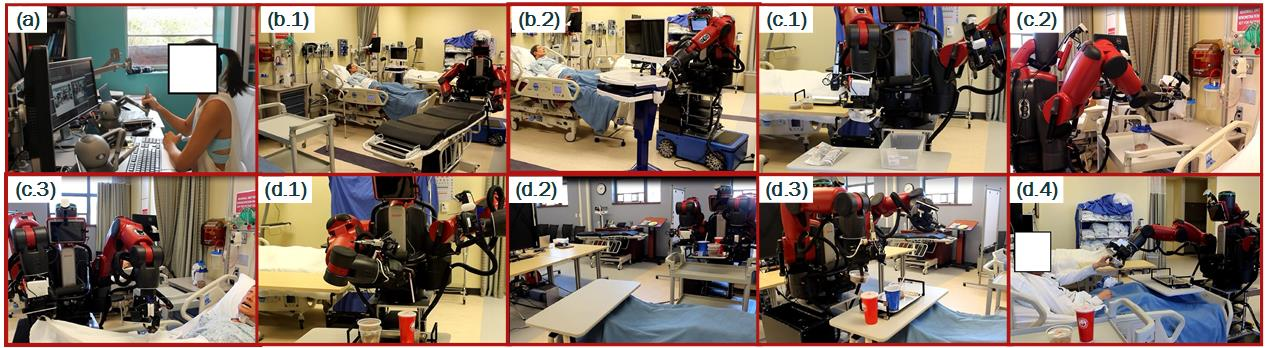
\includegraphics[width=0.99\linewidth]{fig//NursingTask}
\caption{Under (a) direct teleoperation, a mobile humanoid robot tasks can perform complex nursing tasks, including (b.1-2) moving a portable medical devices; (c.1-3) organizing and cleaning the patient's room; and (d.1-4) preparing and serving food to a patient. The manipulation and/or locomotion coordination involved is shared across warehouse, social and in-home assistance scenarios. }
\label{NursingTask}
\vspace{1ex}
\end{figure}
% \end{wrapfigure}

We further propose a novel approach to \underline{evaluate human skill progression} in the training of using different teleoperation interfaces. Our approach grounds in Bernstein's observation that the characteristics that distinguish an expert motor skill are the strong motion regularity that reflects the performance optimization resulted from sufficient practice and refinement, and a small variability to render flexible behavior in the presence of uncertainty. For each teleoperation interface, we extract the motion primitives and task plan of the teleoperated motion coordination, and study their evolution as the teleoperator's skill progresses from novice to expert. Across different teleoperation interfaces, We compare how the teleoperators discover, refine, merge and purge the set of motion primitives and reshape their high-level task plans accordingly. After the teleopertator's skill converge to stable policy and task performance, we further compare the motion coordination strategies in the control of human body and robotic embodiment, to infer the reward function for teleoperated motion coordination. 

This 1-year project will conduct the following three research tasks: 

\begin{itemize}

\item \textbf{Task 1} --- Modeling complex motion coordination of teleoperated robots

% Develop a novel framework to decompose motion coordination to low-level motor skills and high-level task plan; propose modeling methods for coordinated motion primitives and task plan for single robot task and human-robot interaction.   

\item \textbf{Task 2} --- Collecting robot teleoperation data for general-purpose motion coordination tasks  

% Propose novel measurement metrics for evaluating the motion mapping capability of teleoperation interfaces; Compare various teleoperation interfaces for controlling a mobile humanoid to perform general-purpose warehouse tasks that involve complex motion coordination. 

\item \textbf{Task 3} --- Evaluating interface motion mapping capability and teleoperation skill

% Propose novel human performance metrics to evaluate low-level motor skills and high-level task planning skills; study the teleoperation skill progression 

% Develop performance evaluation metrics for human-robot teleoperation system; Study the progression of teleoperated motion coordination from novice to expert, and identify the milestones and thresholds of performance improvement; Investigate the evolution of motion primitives and task plan; Prescribe multi-modality cognitive augmentation to overcome the skill development thresholds; Prescribe physical-cognitive training tasks to develop transferable skills for perception-motion coordination. 

\end{itemize}

\paragraph*{Intellectual Merits}
The intellectual merit of this proposal includes contributions to performance measurement of human-robot collaboration in the teleoperation of complex robotic systems. It proposes a novel measurement framework for evaluating human performance of high-level decision-making and low-level motor skill. It also addresses a critical need in human-robot interface design for evaluation metrics that can quantitatively compare the motion mapping transparency and complexity.

\paragraph*{Broad Impacts}
This project will benefit the teleoperation interface design and evaluation of a broad range of complex robotic systems for warehouse, manufacturing, and maintenance applications. The proposed framework for motion decomposition and performance metrics can be generally applied to measure the worker skill level and progress for industrial, medical, assistance, construction and military tasks, and can be extended to evaluate human skill progression in motor learning and recovery. This project will support one PhD student as research assistant for one year, and one graduate student for 3-month summer research. The research effort will be synergized with graduate and undergraduate courses and develop open-source intuitive teleoperation interface for mobile manipulator robots.  This project will also also involve a team of senior undergrad students working on major qualifying project (MQP), and engage K-12 students through First Robotics and general public in the annually Touch Tomorrow event at WPI.

 
\paragraph*{Qualification of Investigators}
PI Zhi Li has significant experience in tele-robotic systems, including exoskeletons for rehabilitation, tele-surgical robots and tele-nursing robots. Her research focuses on the modeling, planning and learning of complex human and robotic motion coordination, and extended on mechanical design optimization~\cite{li2016design}, robot system integration~\cite{Hauser_Li_TRINA:17}, networked haptics~\cite{li2009networked,li2009remote}, and physical human-robot interaction~\cite{Hauser_Li_BiTelepresence:17}. Related to the proposed project, she has developed the Tele-robotic Intelligent Nursing Assistant (TRINA) system with multi-modal teleoperation interfaces, and conducted system capability evaluation for the direct teleoperation of nursing tasks~\cite{Hauser_Li_TRINA:17}. She is an expert in the regularity and variability of human motion coordination, and human-inspired strategies for controlling kinematically of complex robotic systems~\cite{kim2012resolving,Rosen_Li_EMBC:13,Rosen_Li_IROSChapt:13,Rosen_Li_IROS:14,Rosen_Li_J:14, Rosen_Li:17}. Li's motion learning and prediction algorithm can resolve the kinematic redundancy of a dual-arm rehabilitation exoskeleton, enable it to render arm postures that are fully compatible with healthy operators, and correct abnormal joint coordination due to motor disability. She is also very knowledgeable in human motion skill meassurements~\cite{Rosen_Li_EMBC:15} and human performance in teleoperation~\cite{Hauser_Li_BiTelepresence:17}. 



%-------------------------------------------------------------------------
\section{Background}\label{sec:back}
%-------------------------------------------------------------------------

%-------------------------------------------------------------------------
\subsection{Performance measurement in robot teleoperation}\label{sec:back-performance}
%-------------------------------------------------------------------------
In teleoperation framework, human control a robot through a teleoperation interface to interact with the world. 
Measurement metrics have been developed to evaluate the performance of the four components: human, interface, robot and task, yet these performance metrics haven’t been united in a framework that reflects the adaption level  of human motor control to the physical capability of the robotic system being teleoperated. 
As a result, the performance metrics for human-robot teleoperation system have been developed for each individual component, without little consideration of how they influence each other in a system. For instance, the performance of interface and robot are mostly measured by the motion and perception capability of hardware. Task performance are generally measured completion time and error rate, with domain-specific details. Human performance measurement focuses on the fatigue, stress, attention, and engagement during the tasks. Subjective measurement generally follows the guideline of NASA TXL, while objective performance can measured by or inferred from physiological parameters, kinematic and dynamic motion variables, gaze, muscle and brain activities. 
However, none of these metrics considers human-robot teleoperation as the skill of human using a robotic tool. From this perspective, human performance should be evaluated by the capability of discovering, learning, and refining the motion primitives can be performed by the teleoperated robot, and the capability of task planning and re-planning using the acquired motion primitives. On the other hand, the usability of teleoperation interface should be evaluated by how well it can convey and assist intended human motion and reduce the complexity of controlling motion coordination. 

%-------------------------------------------------------------------------
\subsection{From Teleoperation to Intelligent Assistance}\label{sec:back-intelligent}
%-------------------------------------------------------------------------

Similar to the industrial revolution, task automation has been transforming the interaction and collaboration of human workers and AI agents in healthcare, industry, social service and military tasks. This ``white-collar revolution`` has significantly changed the paradigm of human-robot teleoperation. On one hand, intelligent assistive robots augment the physical and cognitive capabilities of human workers, relieve them from repetitive, tedious, effort-demanding, and dangerous tasks. On the other hand, the-state-of-the-art intelligent robot cannot perform complex and risk-sensitive task without human control. As the tasks for robots increasing with the robot capabilities, teleoperation, with more or less task automation, will remain to be the most reliable way to perform the most difficult tasks. It is also the most efficient way to synergize human-robot performance, and explore and utilize robot physical capability. 
In this context, performance metrics for teleoperation system have been developed to inform interface design and worker skill acquisition process. Robot control interfaces need to provide intelligent assistance to the tasks hard or tedious for direct human control, yet easy, efficient and safe for robot to automate. Study on the robot motion coordination, teleoperated via various teleoperation interface by novice and expert teleoperators, can help to identify such tasks. For routine tasks, motion coordination can be learned and automated through the combination of imitation and reinforcement learning. For free-style tasks, robot teleoperators have been assisted with motion smoothing and scaling to improve their precision control, and with power augmentation in labor-demanding work. Little research has considered reducing the control effort by automating secondary tasks and the control of the redundant degrees of freedom in motion coordination. 

%-------------------------------------------------------------------------
\subsection{Adaption of Human Motor Control to Robotic Physical Embodiment}\label{sec:back-intelligent}
%-------------------------------------------------------------------------
The control effort-sharing between robot automation and direct human control can refer to how human motor system regulate the controlled and uncontrolled manifolds. Take reaching-to-grasp motion for instance, as human focusing on control hand position and orientation, the arm posture (i.e., how to pose the elbow) is automatically handled. In bimanual coordination, human focuses more on the control of dominant hand, while dominant hand follows naturally and accordingly. Intelligent robot control interface needs to automate these naturally uncontrolled and secondary tasks, particularly for complex robotic systems. Providing such intelligent assistance also reduce the learning efforts in teleoperation skill acquisition. Learning to control a robot through teleoperation interface is essentially a process of adapting human motor control to a robot physical embodiment. Ideally, a teleoperation interface should minimize the adaption efforts. One way to achieve that is to ensure the motion coordination rendered under shared autonomous control comply with the high-level motion control strategy of human motion. These high-level motion control strategies are abstract from human/robot physical embodiment (unlike the low-level coordination such as joint coupling), and reflect the rationality of how physical structure, perception and motion control synergize with each other. The high-level coordination strategies that involve both robot motion and perception haven’t well-studied. Related work on human motion coordination (e.g., arm redundancy, arm-hand coordination, synergy in hand motion, gait cycle and whole-body coordination in locomotion, etc), robot motion coordination (e.g., coordination of macro-micro manipulators, mobile manipulator robots, humanoid robot, etc), and interactive-perception can be united to enhance the understanding. 

% %-------------------------------------------------------------------------
% \subsection{PI's related work}\label{sec:back-PI}
% %-------------------------------------------------------------------------



%-------------------------------------------------------------------------
\section{Research Plan}\label{sec:plan}
%-------------------------------------------------------------------------

%-------------------------------------------------------------------------
\subsection{Modeling of Teleoperated Robot Motion Coordination}\label{sec:plan-modeling}
%-------------------------------------------------------------------------

%-------------------------------------------------------------------------
\subsubsection{Modeling low-level motion coordination}\label{sec:plan-modeling-MP}
%-------------------------------------------------------------------------

\paragraph*{Parameterized models for low-level motion skills} Motor primitives are the building blocks of complex and goal-directed motor skills~\cite{flash2005motor}. Inspired by human motor primitives, dynamic movement primitives (DMP) were proposed for learning and producing episodic and rhythmic motions of spatial and temporal coordination~\cite{ijspeert2013dynamical}. More recently, probabilistic modeling of motion primitives has been proposed to better address demonstration regularity and variability for imitation learning~\cite{calinon2007learning,calinon2010learning}, to account for sensing uncertainty in the feedback loop control for motion reproduction~\cite{meier2016probabilistic}, and to model the temporal and spatial dependency of human-robot interaction ~\cite{maeda2017phase}. Beyond the field of imitation learning, constructing parameterized action/motion primitives has also been investigated by the robotic control \cite{fu2013bottom} and reinforcement learning (RL) communities \cite{masson2016reinforcement}. Different from motion primitives derived using Gaussian basis regression, a parameterized action is a discrete action parameterized by a real-valued vector. For example, a navigation controller is an action that is parameterized by a goal position. For a given parameter, a low-level optimal control/motion plan can be generated. Recent work proposes a RL algorithm to simultaneously learn both the optimal parameter and the low-level policy in Markov decision processes \cite{masson2016reinforcement}. However, such an episodic approach does not address spatial and temporal dependency between a set of parameterized actions. 

\paragraph*{Autonomous Motion Segmentation}



\paragraph*{Learning motion primitives from demonstrations}
The demonstrations are collected from a mobile humanoid robot controlled through various teleoperation interfaces. Standard human and robot performance metrics are used to evaluate meta performance of human-robot teleoperation system, and quantify the skill levels of novices and experts. Dynamic movement primitives (DMP) and Gaussian Mixture Model/Gaussian Mixture Regression (GMM/GMR) can used to model the motion coordination within robotic system, while Probabilistic Movement Primitives (Pro-MP) is used to model the motion coordination between robotic system and environment.

\begin{itemize}
    \item DMP
    
    \item GMM/GMR
    
    \item Pro-MP
    
\end{itemize}

\paragraph*{Learning the structure of motion primitive sets}

Human-driven classification: 

- Associate MP to robot component - hand, arm, base

- Associate MP to interface control mode

- Associate MP to motion type -- Reaching, Grasping and Locomotion Primitives

- Coupling MP of different components through shared object, task goal? 

Unsupervised learning -- Clustering MP

%-------------------------------------------------------------------------
\subsubsection{Modeling of high-level task Structure}\label{sec:plan-modeling-Plan}
%-------------------------------------------------------------------------

\paragraph{Abstract representation of robot task} The teleoperated robot tasks we consider consist of many inter-dependent procedures and complex state-action relationships. Thus, it is useful to learn abstract task structures from the demonstrations of human experts to facilitate task reasoning, decomposition, and reproduction. Previous research in robot learning has used high-level task structure representations such as Finite-State Automaton (FSA)~\cite{niekum2013semantically}, skill trees~\cite{konidaris2012robot}, and semi-Markov decision process~\cite{konidaris2018skills}. A high-level task plan can be built upon low-level motion primitives~\cite{konidaris2012robot} and symbolic representations of states and actions~\cite{konidaris2018skills}. 

We consider three abstract representations for task plan, which will lead to different task plan evaluation metrics: 


\paragraph*{Learning task plan as skill tree}


\paragraph*{Learning task plan as Semi-Markov Decision Process} Abstract task structure can be composed using symbols for actions and states. At a high-level, a teleoperated robot task structure is a semi-Markov decision process built upon the symbolic representations for the states and the actions induced state transitions. In addition, uncertainty in action can be captured with probabilistic automata. Both the action and state symbols are associated to the teleoperated robot, while the (passive) objects being manipulated are only associated with state symbols. The action symbols are abstract representation of compatible motion primitives, while the state symbols are probabilistic distributions of robot/object states learned directly from robot sensorimotor data. To relate an action to object states, we observe from the demonstrations the probabilistic distributions that describe the effects of the action. Note that the single-agent framework in~\cite{konidaris2018skills} is not sufficient to address the task complexity in multilateral teleoperation, which enables multiple teleoperators to (simultaneously) control different components of the same robotic system. Future work also needs to this framework to encompass the collaboration between a teleoperated robot and remote human collaborator. 

% Learning first order task logic


\paragraph*{Learning task plan as Probabilistic Finite-state Automaton}

% Learning high-order and temporal task logic


%-------------------------------------------------------------------------
\subsection{Comparing Teleoperation Interfaces for mobile manipulator robot}\label{sec:plan-interface}
%-------------------------------------------------------------------------

%-------------------------------------------------------------------------
\subsubsection{Platform and Preliminary work}\label{sec:plan-interface-hardware}
%-------------------------------------------------------------------------

%-------------------------------------------------------------------------
\subsubsection{Measurement metrics}\label{sec:plan-interface-metrics}
%-------------------------------------------------------------------------

%-------------------------------------------------------------------------
\subsubsection{Experiment design}\label{sec:plan-interface-exp}
%-------------------------------------------------------------------------

\paragraph{Task description}


\paragraph{Subjects}


\paragraph{Research Hypotheses}


\paragraph{Data collection and analysis}

%-------------------------------------------------------------------------
\subsection{The Development of Robot Teleoperation skill }\label{sec:plan-skill}
%-------------------------------------------------------------------------

%-------------------------------------------------------------------------
\subsubsection{Evaluating low-level motor skills}\label{sec:plan-skill-low}
%-------------------------------------------------------------------------

%-------------------------------------------------------------------------
\subsubsection{Evaluating high-level task planning}\label{sec:plan-skill-high}
%-------------------------------------------------------------------------

%-------------------------------------------------------------------------
\subsubsection{Experiment Design}\label{sec:plan-skill-exp}
%-------------------------------------------------------------------------

\paragraph{Subjects}

\paragraph{Tasks}

\paragraph{Research Hypotheses}


\paragraph{Data collection and analysis}


% Extended from the , our high-level task representation considers the effects that can only be achieved by joint human-robot action, and the effects that can be achieved by either the human or the robot. It generalizes to probabilistic transitions to capture several possible next steps given the current action and state of human (robot), and the uncertainty in dynamic task assignment. For example, a nurse may takeover the task step of the robot under certain circumstances. The abstract representation we propose is more inclusive and flexible since it encompasses the individual human/robot tasks and robot-mediated collaboration scenarios. 



% % We also observe if there exist correlation between the actions of end user and teleoperated robot to determine the coordinated motions should be modeled using interactive or independent motion primitives. 
% Here we provide more details on automata learning. Generally speaking, abstraction-based learning seeks to infer the abstract language $L$ that describes  a set of task sequences from collaborative human experts, referred to as the \emph{language of the teleoperation system}. During interactions, the autonomous system only observes finitely many instances from this language and the goal is to generalize from such observed high-level task sequences to an automaton or grammar representation of the language that may include infinitely many possible task sequences. For this task, grammatical inference (GI) \cite{de2010grammatical}, also known as automata learning, is appropriate as an abstraction-based learning mechanism. GI is a class of algorithms that generalize from a finite number of sentences to provide a grammar that describes the language, which may contain infinitely many words. As an example, consider the tele-operated robot accomplishes two tasks:  ``\textbf{P}ick up the cup (P) and \textbf{H}and it over to the nurse (H)'', and 
% ``\textbf{M}ove to the table (M), \textbf{P}ick up the cup and pla\textbf{C}e it on the shelf, and pick up the bag and hand it over to the nurse.'' These two task sequences generate a \emph{prefix}-tree, similar to a skill tree \cite{konidaris2018skills} in Fig.~\ref{fig:gi} (a) that accepts exactly two words, i.e., task sequences. Using the state merging operation \cite{de2010grammatical} in the GI algorithm, the system is able to generalize to the automaton in Fig.~\ref{fig:gi} (b), and understand it can pick and place objects infinitely often, indicated by the loop. Lastly, with another state merging, the robot learns it is able to relocate to different positions with action ``M'' (move), and can pick and place an object or hand an object over to the nurse. Using the inference algorithm, the automaton learned by GI generalizes from a skill tree to an automaton or grammar that represents a potentially infinite set of possible task decompositions and task sequences.


% \begin{figure}[t!]
%     \centering
%     \begin{subfigure}[b]{0.4\textwidth}
%         \centering
% 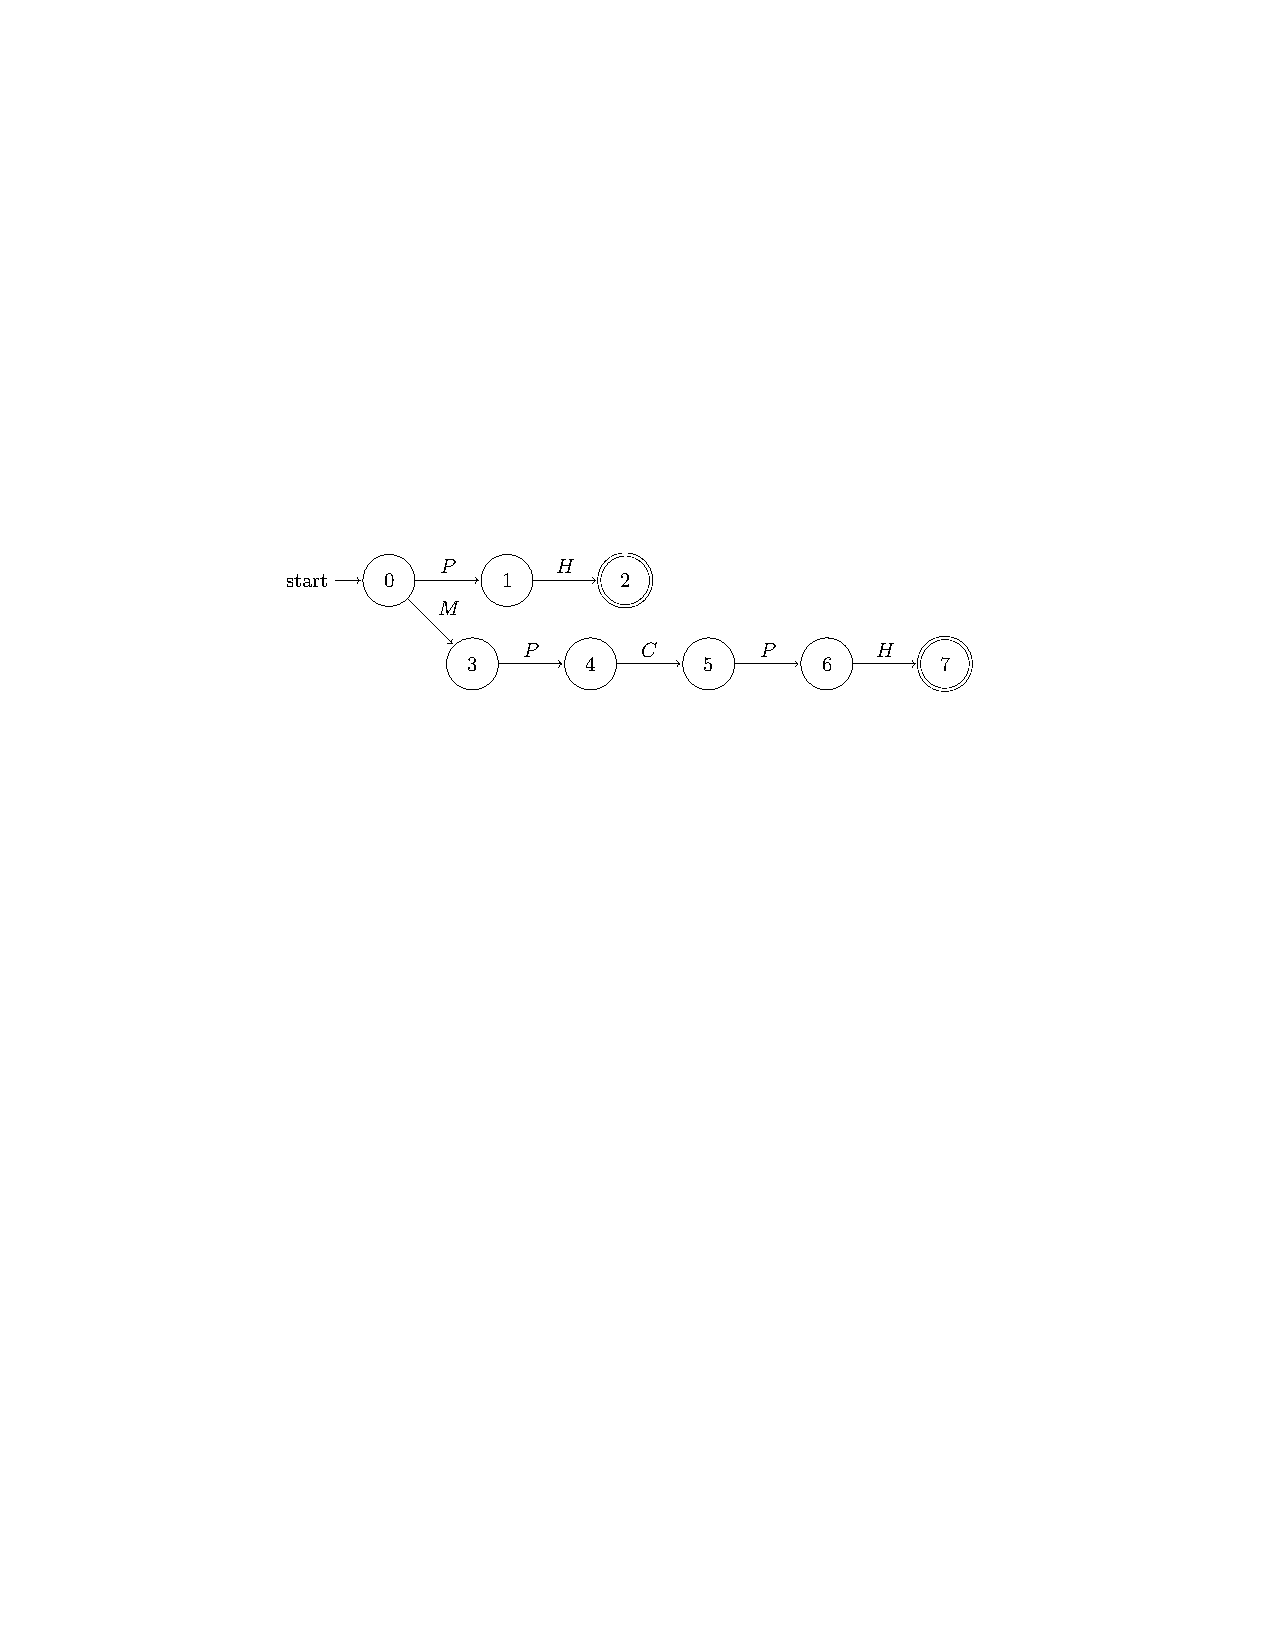
\includegraphics[width=\textwidth]{fig/original.pdf}        \caption{}
%     \end{subfigure}%
%     \begin{subfigure}[b]{0.3\textwidth}
%         \centering
% 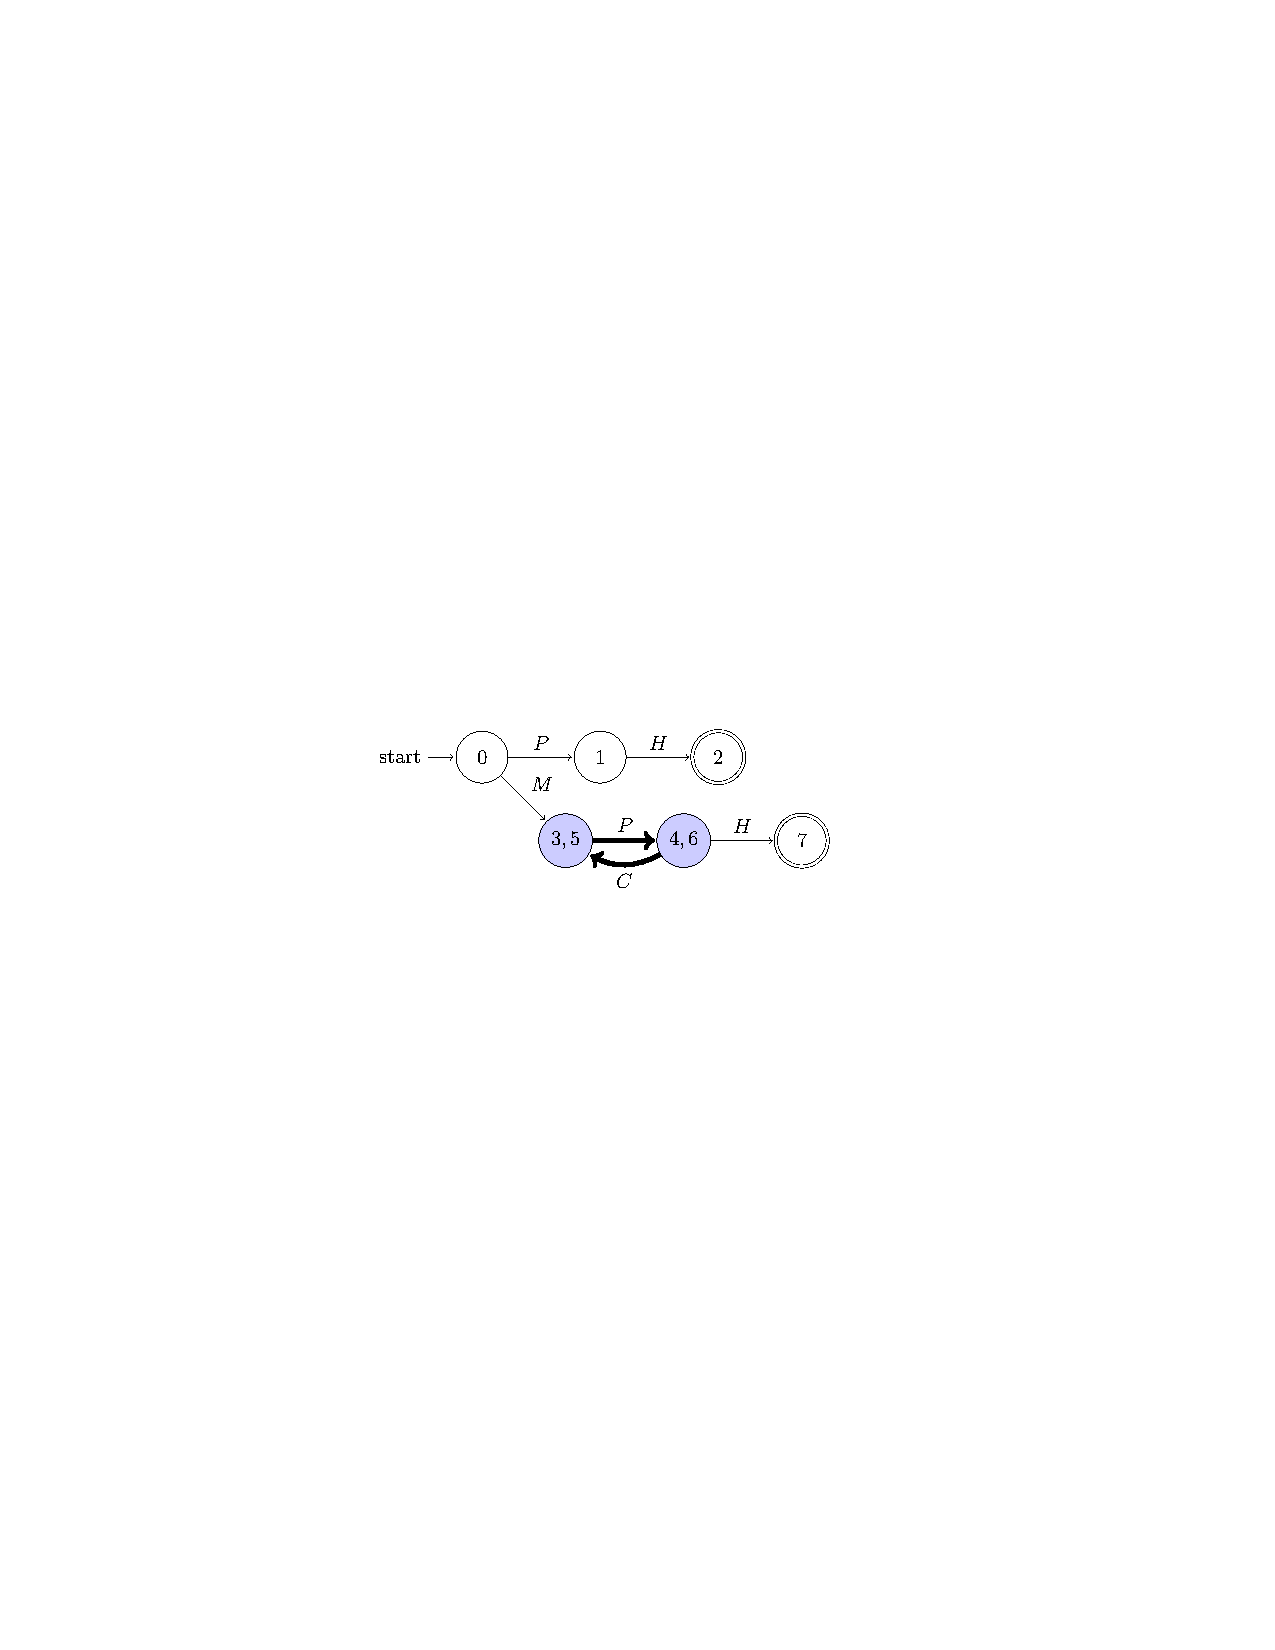
\includegraphics[width=\textwidth]{fig/merge1.pdf}         \caption{}
%     \end{subfigure}%
%     \begin{subfigure}[b]{0.28\textwidth}
%         \centering
% 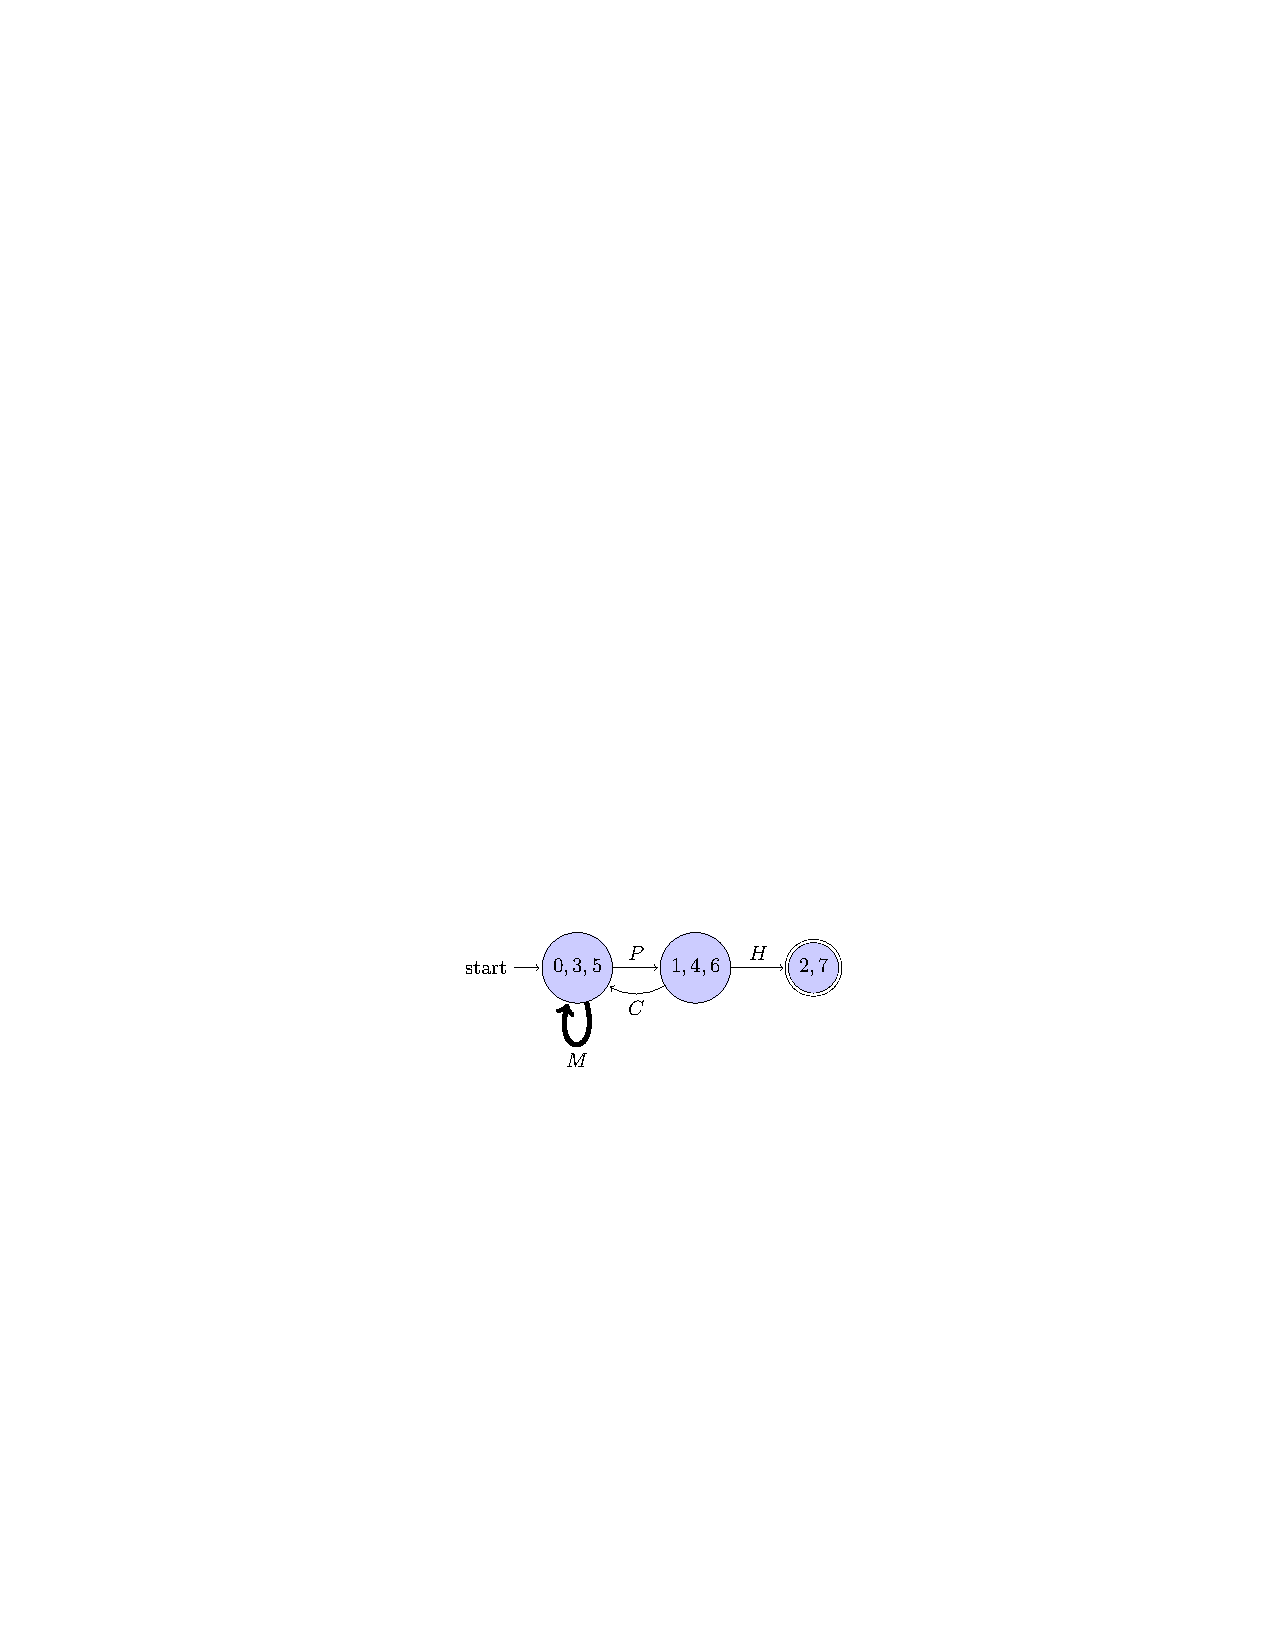
\includegraphics[width=\textwidth]{fig/merge2.pdf}     
% \caption{}\end{subfigure}
%     \caption{An illustration of the grammatical inference algorithm using state merging. (a) is the original prefix tree/skill tree. (b) generalizes (a) by merging state $3,5$ and $4,6$. (c) further generalizes (b) by merging $0,3,5$, $1,4,6$, and $2,7$. The state merging or splitting is guided by a GI algorithm selected for the target language on positive data only, or with both positive and negative data.}
%     \label{fig:gi}
% \end{figure}


% In this specific application context, we will consider several GI algorithms, including learning from positive demonstration under the assumption that actions have pairwise dependence \cite{heinz2013learning}, and the $L^\ast$ algorithm, which learns from both positive and negative demonstrations \cite{angluin1987learning}, given that negative demonstrations may be obtained from the nurses’ feedback of unreasonable behavior. We propose to learn, for three interacting agents, their individual alphabets and languages. We seperate the concern of  action synchronization, conflict, and sequencing from learning and propose to capture such constraints for collaboration and coordination through product operations between languages/automata, including but not limited to, synchronization composition and sequential composition \cite{alur2015principles,hopcroft2001introduction}. 
% For instance, synchronization will enable us to capture the dependency between the action of aiming the camera at the hand of the human nurse with the reaching motion of the manipulator.  Inference algorithms for probabilistic finite-state automata \cite{clark2004pac} \cite[Chap 12]{de2010grammatical} will further enable us to capture stochastic transitions resulting from uncertain outcomes of actions and uncertainty in task step coordination. 


% % adapt human motion coordination strategies to their remote robot surrogates.

% To meet this need, we propose to learn from novice- and expert-demonstration of the motion coordination, compare the demonstrations by their low-level motion primitive models and high-level motion plan model, to learn the features for measure the performance of human-robot teleoperation system. The demonstrations are collected from a mobile humanoid robot controlled through various teleoperation interfaces. Standard human and robot performance metrics are used to evaluate meta performance of human-robot teleoperation system, and quantify the skill levels of novices and experts. Dynamic movement primitives (DMP) and Gaussian Mixture Model/Gaussian Mixture Regression (GMM/GMR) are used to model the motion coordination within robotic system, while Probabilistic Movement Primitives (Pro-MP) is used to model the motion coordination between robotic system and environment. Novel metrics for the regularity, variability, complexity of the motion primitives are proposed as the features to characterize the low-level motor skills. Machine learning methods are used to identify the principle components and characteristic synergy in the motion primitive feature space, to compare low-level motor skills across tasks, teleoperation interfaces, and users. To model the high-level task plan, we abstract the critical robot states in motion coordination  and motion primitives for state transition to symbols, and use these symbols to construct an abstract task space graph. The costs of graph nodes and edges, which denote the abstract states and state-transition motion primitives, are assigned by weighting the teleoperator's operation efforts, efficiency, frequency and success ratio. Given the abstract motion coordination representation, we propose several optimization criteria, derived from several hypotheses of the human motion coordination strategies, and compose a reward function with unknown weighting coefficients. The weighting assignment learned from demonstrated high-level task plan can be used for evaluate and compare a teleoperator's motion coordination control strategies. 

% 





% Take the teleoperation of mobile humanoid nursing robot for instance: the motion coordination involved in patient-caring tasks includes , and may extend to the coordination of end-effectors for sensing and action. 

% skill acquisition efforts of novice worker to  

% Tele-operated robotic systems extend the physical capabilities of medical and industrial workers to perform  tasks in remote, inaccessible, and/or hazardous environments. 

% tasks that require human-level manipulation dexterity and decision-making intelligence are infeasible through autonomous control, yet can be accomplished under direct (tele)operation. To freely and efficiently control their remote surrogates, human workers need to devote significant efforts to learn the motion and perception mapping defined by the (tele)operation interface. To address this needs, we propose to investigate the physical and cognitive interactions between human workers and (tele)operation interfaces, and develop a user interface to support intuitive robot control and multi-modality cognitive augmentation. Our proposed project aims to (a) reduce the teleoperation control effort in dexterous and coordinated manipulation tasks, and to (b) facilitate novice workers to acquire the fine motor skills for operating complicate robotic systems to work on various manufacturing tasks. To this end, we propose to investigate theories and technologies that (1) Shift the boundary between direct teleoperation and autonomous control based on the physical and mental status of the operator, (2) Infer human teleoperator's contextual intent based on the knowledge of manipulation tasks and human motions, in order to automate low-level robot actions. 

% \vspace{0.5 em}

% \paragraph*{\Large Intellectual Merit}
% This project addresses how multi-modality cognitive feedback affects human motor behavior and motor learning process. Specifically, we will experimentally study in teleoperated manipulation tasks that requires simultaneous control of multiple robot components, such as loco-manipulation, bimanual coordination, arm-hand-finger coordination. For \textbf{expert workers}, we focuses on \textit{how human decision-making and task operation can be affected by single- and multi-modality cognitive feedback, and investigate methods for intuitive and integrated representation of task information and cognitive feedback}. For \textbf{novice workers}, we will focus on \textit{how multi-modality cognitive feedback affects the explicit and implicit learning of dexterous and coordinated manipulation motor skills}, as well as \textit{when and how to provide high-level/abstract cognitive feedback (e.g., verbal/text instructions, numbers, etc.) and low-level intuitive cognitive feedback (e.g., colors, shapes, sounds, tactile and forces, etc.) to facilitate the interactive and associated explicit and implicit motor learning}. Our proposed research is unique for it will develop a unified framework that integrate the model-based and model-less robot learning methodologies to reveal the underlying principles of the associated implicit and explicit human motor learning processes. The enhanced understanding of the cognitive and physical interactions between human worker and teleoperation interfaces further leads to novel techniques for user-adaptive cognitive augmentation and decision-making assistance, which leverages ``cloud wisdom'' and adjust the human-robot control efforts based on a human worker's intents, physical/mental states, and skill level. 

% % to robot learning that acquire motion and task knowledge through  (e.g., reinforcement learning with explicit reward function v.s. learning through convolutional neural network). Inspired by how human can develop situational awareness and motor skills through intuitive and abstract cognitive feedback and augmentation, we will further develop novel robot teaching methodologies for that leverage human-guided robot interactions with environments and demonstrations/critiques from human teachers. 



%-------------------------------------------------------------------------
\section{Broader Impact}\label{sec:impact}
%-------------------------------------------------------------------------

\paragraph{Broader Applications} This project will benefit the interface design and evaluation of a broad range of complex tele-robotic systems, including mobile manipulator robots, humanoids, multi-arm manipulator system, and multi-agent robots. The proposed human performance metrics can be generally applied to evaluate the robot operation skill for industrial, medical, social and in-home assistance, construction, space and military tasks. It also provides a framework for evaluating the skill development of general-purpose motor tasks and motor recovery in rehabilitation.  

\paragraph{Research-Education Synergy} This project will synergize research effort with graduate and undergraduate education in robotics engineering on human-robot interaction and industrial robotics at WPI. This project will support one PhD student as research assistant, to work on the experimental study on teleoperation interface comparison and teleoperation skill progression. It will involve a second graduate student for 3-month summer research to assist data analysis and improve the robot teleoperation interface with multi-model cognitive augmentation. This project will provide hand-on projects to a graduate course (RBE 595 --- Synergy of Human and Robotic System) offered to students with robotics engineering program, and a undergraduate courses (RBE/ME/MFE 4815 --- Industrial Robotics) offer to students with robotics, mechanical and manufacturing engineering. It will also offer project and platform to inter-disciplinary major qualifying project (MQP) for senior undergraduate student with the college of engineering at WPI. Through this MQP we will develop a 3D printed, customizable robot teleoperation interface for intuitive control of mobile manipulator robots. The MQP project outcome will be shared as open-source CAD model and ROS-compatible software package. This project will engage K-12 students through First Robotics and general public in the annually Touch Tomorrow event at WPI.

\paragraph{Potential Future Work} The proposed project is primarily concerned of teleoperating mobile humanoid robots to perform low-precision motion coordination tasks. Future work will be extended to the teleoperation of multi-robot system for high-precision tasks (e.g., surgery and cable-tie tasks), and of large number of robots (e.g., swarm robots). The implementation and system evaluation can be conducted on the multi-arm surgical robot platform available at WPI AIM lab, swarm robot system available at WPI NEST lab, and industrial robot platform available at NIST research labs. Our future work will extend framework for motion and task modeling to encompass the scenario of multi-lateral teleoperation --- which enable multiple teleoperators to (simultaneously) control different components of a robotic system.  We will also develop robot control interface that provides intelligent assistance that automate the task components different for direct teleoperation control, and shift the control between human teleoperator and intelligent tele-operated robot based human skill and fatigue level. 


\pagebreak
\setcounter{page}{1}
\bibliographystyle{IEEEtran}
\bibliography{./ZhiLi_ref}

\end{document}
